
%% bare_conf.tex
%% V1.4b
%% 2015/08/26
%% by Michael Shell
%% See:
%% http://www.michaelshell.org/
%% for current contact information.
%%
%% This is a skeleton file demonstrating the use of IEEEtran.cls
%% (requires IEEEtran.cls version 1.8b or later) with an IEEE
%% conference paper.
%%
%% Support sites:
%% http://www.michaelshell.org/tex/ieeetran/
%% http://www.ctan.org/pkg/ieeetran
%% and
%% http://www.ieee.org/

%%*************************************************************************
%% Legal Notice:
%% This code is offered as-is without any warranty either expressed or
%% implied; without even the implied warranty of MERCHANTABILITY or
%% FITNESS FOR A PARTICULAR PURPOSE! 
%% User assumes all risk.
%% In no event shall the IEEE or any contributor to this code be liable for
%% any damages or losses, including, but not limited to, incidental,
%% consequential, or any other damages, resulting from the use or misuse
%% of any information contained here.
%%
%% All comments are the opinions of their respective authors and are not
%% necessarily endorsed by the IEEE.
%%
%% This work is distributed under the LaTeX Project Public License (LPPL)
%% ( http://www.latex-project.org/ ) version 1.3, and may be freely used,
%% distributed and modified. A copy of the LPPL, version 1.3, is included
%% in the base LaTeX documentation of all distributions of LaTeX released
%% 2003/12/01 or later.
%% Retain all contribution notices and credits.
%% ** Modified files should be clearly indicated as such, including  **
%% ** renaming them and changing author support contact information. **
%%*************************************************************************


% *** Authors should verify (and, if needed, correct) their LaTeX system  ***
% *** with the testflow diagnostic prior to trusting their LaTeX platform ***
% *** with production work. The IEEE's font choices and paper sizes can   ***
% *** trigger bugs that do not appear when using other class files.       ***                          ***
% The testflow support page is at:
% http://www.michaelshell.org/tex/testflow/



\documentclass[conference]{IEEEtran}
% Some Computer Society conferences also require the compsoc mode option,
% but others use the standard conference format.
%
% If IEEEtran.cls has not been installed into the LaTeX system files,
% manually specify the path to it like:
% \documentclass[conference]{../sty/IEEEtran}


% Some very useful LaTeX packages include:
% (uncomment the ones you want to load)

% *** OWN PACKAGES ***
% Nach LaTex Dokument Hellmich & Espinoza
\usepackage[utf8]{inputenc} % für Umlaute im Dokument
\usepackage[ngerman]{babel} % für deutsche Silbentrennung


% *** MISC UTILITY PACKAGES ***
%
%\usepackage{ifpdf}
% Heiko Oberdiek's ifpdf.sty is very useful if you need conditional
% compilation based on whether the output is pdf or dvi.
% usage:
% \ifpdf
%   % pdf code
% \else
%   % dvi code
% \fi
% The latest version of ifpdf.sty can be obtained from:
% http://www.ctan.org/pkg/ifpdf
% Also, note that IEEEtran.cls V1.7 and later provides a builtin
% \ifCLASSINFOpdf conditional that works the same way.
% When switching from latex to pdflatex and vice-versa, the compiler may
% have to be run twice to clear warning/error messages.






% *** CITATION PACKAGES ***
%
%\usepackage{cite}
% cite.sty was written by Donald Arseneau
% V1.6 and later of IEEEtran pre-defines the format of the cite.sty package
% \cite{} output to follow that of the IEEE. Loading the cite package will
% result in citation numbers being automatically sorted and properly
% "compressed/ranged". e.g., [1], [9], [2], [7], [5], [6] without using
% cite.sty will become [1], [2], [5]--[7], [9] using cite.sty. cite.sty's
% \cite will automatically add leading space, if needed. Use cite.sty's
% noadjust option (cite.sty V3.8 and later) if you want to turn this off
% such as if a citation ever needs to be enclosed in parenthesis.
% cite.sty is already installed on most LaTeX systems. Be sure and use
% version 5.0 (2009-03-20) and later if using hyperref.sty.
% The latest version can be obtained at:
% http://www.ctan.org/pkg/cite
% The documentation is contained in the cite.sty file itself.






% *** GRAPHICS RELATED PACKAGES ***
%
\ifCLASSINFOpdf
  % \usepackage[pdftex]{graphicx}
  % declare the path(s) where your graphic files are
  % \graphicspath{{../pdf/}{../jpeg/}}
  % and their extensions so you won't have to specify these with
  % every instance of \includegraphics
  % \DeclareGraphicsExtensions{.pdf,.jpeg,.png}
\else
  % or other class option (dvipsone, dvipdf, if not using dvips). graphicx
  % will default to the driver specified in the system graphics.cfg if no
  % driver is specified.
  % \usepackage[dvips]{graphicx}
  % declare the path(s) where your graphic files are
  % \graphicspath{{../eps/}}
  % and their extensions so you won't have to specify these with
  % every instance of \includegraphics
  % \DeclareGraphicsExtensions{.eps}
\fi
% graphicx was written by David Carlisle and Sebastian Rahtz. It is
% required if you want graphics, photos, etc. graphicx.sty is already
% installed on most LaTeX systems. The latest version and documentation
% can be obtained at: 
% http://www.ctan.org/pkg/graphicx
% Another good source of documentation is "Using Imported Graphics in
% LaTeX2e" by Keith Reckdahl which can be found at:
% http://www.ctan.org/pkg/epslatex
%
% latex, and pdflatex in dvi mode, support graphics in encapsulated
% postscript (.eps) format. pdflatex in pdf mode supports graphics
% in .pdf, .jpeg, .png and .mps (metapost) formats. Users should ensure
% that all non-photo figures use a vector format (.eps, .pdf, .mps) and
% not a bitmapped formats (.jpeg, .png). The IEEE frowns on bitmapped formats
% which can result in "jaggedy"/blurry rendering of lines and letters as
% well as large increases in file sizes.
%
% You can find documentation about the pdfTeX application at:
% http://www.tug.org/applications/pdftex





% *** MATH PACKAGES ***
%
%\usepackage{amsmath}
% A popular package from the American Mathematical Society that provides
% many useful and powerful commands for dealing with mathematics.
%
% Note that the amsmath package sets \interdisplaylinepenalty to 10000
% thus preventing page breaks from occurring within multiline equations. Use:
%\interdisplaylinepenalty=2500
% after loading amsmath to restore such page breaks as IEEEtran.cls normally
% does. amsmath.sty is already installed on most LaTeX systems. The latest
% version and documentation can be obtained at:
% http://www.ctan.org/pkg/amsmath





% *** SPECIALIZED LIST PACKAGES ***
%
%\usepackage{algorithmic}
% algorithmic.sty was written by Peter Williams and Rogerio Brito.
% This package provides an algorithmic environment fo describing algorithms.
% You can use the algorithmic environment in-text or within a figure
% environment to provide for a floating algorithm. Do NOT use the algorithm
% floating environment provided by algorithm.sty (by the same authors) or
% algorithm2e.sty (by Christophe Fiorio) as the IEEE does not use dedicated
% algorithm float types and packages that provide these will not provide
% correct IEEE style captions. The latest version and documentation of
% algorithmic.sty can be obtained at:
% http://www.ctan.org/pkg/algorithms
% Also of interest may be the (relatively newer and more customizable)
% algorithmicx.sty package by Szasz Janos:
% http://www.ctan.org/pkg/algorithmicx




% *** ALIGNMENT PACKAGES ***
%
%\usepackage{array}
% Frank Mittelbach's and David Carlisle's array.sty patches and improves
% the standard LaTeX2e array and tabular environments to provide better
% appearance and additional user controls. As the default LaTeX2e table
% generation code is lacking to the point of almost being broken with
% respect to the quality of the end results, all users are strongly
% advised to use an enhanced (at the very least that provided by array.sty)
% set of table tools. array.sty is already installed on most systems. The
% latest version and documentation can be obtained at:
% http://www.ctan.org/pkg/array


% IEEEtran contains the IEEEeqnarray family of commands that can be used to
% generate multiline equations as well as matrices, tables, etc., of high
% quality.




% *** SUBFIGURE PACKAGES ***
%\ifCLASSOPTIONcompsoc
%  \usepackage[caption=false,font=normalsize,labelfont=sf,textfont=sf]{subfig}
%\else
%  \usepackage[caption=false,font=footnotesize]{subfig}
%\fi
% subfig.sty, written by Steven Douglas Cochran, is the modern replacement
% for subfigure.sty, the latter of which is no longer maintained and is
% incompatible with some LaTeX packages including fixltx2e. However,
% subfig.sty requires and automatically loads Axel Sommerfeldt's caption.sty
% which will override IEEEtran.cls' handling of captions and this will result
% in non-IEEE style figure/table captions. To prevent this problem, be sure
% and invoke subfig.sty's "caption=false" package option (available since
% subfig.sty version 1.3, 2005/06/28) as this is will preserve IEEEtran.cls
% handling of captions.
% Note that the Computer Society format requires a larger sans serif font
% than the serif footnote size font used in traditional IEEE formatting
% and thus the need to invoke different subfig.sty package options depending
% on whether compsoc mode has been enabled.
%
% The latest version and documentation of subfig.sty can be obtained at:
% http://www.ctan.org/pkg/subfig




% *** FLOAT PACKAGES ***
%
%\usepackage{fixltx2e}
% fixltx2e, the successor to the earlier fix2col.sty, was written by
% Frank Mittelbach and David Carlisle. This package corrects a few problems
% in the LaTeX2e kernel, the most notable of which is that in current
% LaTeX2e releases, the ordering of single and double column floats is not
% guaranteed to be preserved. Thus, an unpatched LaTeX2e can allow a
% single column figure to be placed prior to an earlier double column
% figure.
% Be aware that LaTeX2e kernels dated 2015 and later have fixltx2e.sty's
% corrections already built into the system in which case a warning will
% be issued if an attempt is made to load fixltx2e.sty as it is no longer
% needed.
% The latest version and documentation can be found at:
% http://www.ctan.org/pkg/fixltx2e


%\usepackage{stfloats}
% stfloats.sty was written by Sigitas Tolusis. This package gives LaTeX2e
% the ability to do double column floats at the bottom of the page as well
% as the top. (e.g., "\begin{figure*}[!b]" is not normally possible in
% LaTeX2e). It also provides a command:
%\fnbelowfloat
% to enable the placement of footnotes below bottom floats (the standard
% LaTeX2e kernel puts them above bottom floats). This is an invasive package
% which rewrites many portions of the LaTeX2e float routines. It may not work
% with other packages that modify the LaTeX2e float routines. The latest
% version and documentation can be obtained at:
% http://www.ctan.org/pkg/stfloats
% Do not use the stfloats baselinefloat ability as the IEEE does not allow
% \baselineskip to stretch. Authors submitting work to the IEEE should note
% that the IEEE rarely uses double column equations and that authors should try
% to avoid such use. Do not be tempted to use the cuted.sty or midfloat.sty
% packages (also by Sigitas Tolusis) as the IEEE does not format its papers in
% such ways.
% Do not attempt to use stfloats with fixltx2e as they are incompatible.
% Instead, use Morten Hogholm'a dblfloatfix which combines the features
% of both fixltx2e and stfloats:
%
% \usepackage{dblfloatfix}
% The latest version can be found at:
% http://www.ctan.org/pkg/dblfloatfix




% *** PDF, URL AND HYPERLINK PACKAGES ***
%
%\usepackage{url}
% url.sty was written by Donald Arseneau. It provides better support for
% handling and breaking URLs. url.sty is already installed on most LaTeX
% systems. The latest version and documentation can be obtained at:
% http://www.ctan.org/pkg/url
% Basically, \url{my_url_here}.




% *** Do not adjust lengths that control margins, column widths, etc. ***
% *** Do not use packages that alter fonts (such as pslatex).         ***
% There should be no need to do such things with IEEEtran.cls V1.6 and later.
% (Unless specifically asked to do so by the journal or conference you plan
% to submit to, of course. )


% correct bad hyphenation here
\hyphenation{op-tical net-works semi-conduc-tor}


\begin{document}
%
% paper title
% Titles are generally capitalized except for words such as a, an, and, as,
% at, but, by, for, in, nor, of, on, or, the, to and up, which are usually
% not capitalized unless they are the first or last word of the title.
% Linebreaks \\ can be used within to get better formatting as desired.
% Do not put math or special symbols in the title.
\title{Über die Automatisierbarkeit von Traceability im Requirements Engineering\\ - ein systematischer Literatur Review}


% author names and affiliations
% use a multiple column layout for up to three different
% affiliations
\author{\IEEEauthorblockN{Patrick Reif}
\IEEEauthorblockA{Hochschule Bonn-Rhein-Sieg\\Fachbereich Informatik\\Sankt Augustin}}
%\and
%\IEEEauthorblockN{Homer Simpson}
%\IEEEauthorblockA{Twentieth Century Fox\\
%Springfield, USA\\
%Email: homer@thesimpsons.com}
%\and
%\IEEEauthorblockN{James Kirk\\ and Montgomery Scott}
%\IEEEauthorblockA{Starfleet Academy\\
%San Francisco, California 96678--2391\\
%Telephone: (800) 555--1212\\
%Fax: (888) 555--1212}}

% conference papers do not typically use \thanks and this command
% is locked out in conference mode. If really needed, such as for
% the acknowledgment of grants, issue a \IEEEoverridecommandlockouts
% after \documentclass

% for over three affiliations, or if they all won't fit within the width
% of the page, use this alternative format:
% 
%\author{\IEEEauthorblockN{Michael Shell\IEEEauthorrefmark{1},
%Homer Simpson\IEEEauthorrefmark{2},
%James Kirk\IEEEauthorrefmark{3}, 
%Montgomery Scott\IEEEauthorrefmark{3} and
%Eldon Tyrell\IEEEauthorrefmark{4}}
%\IEEEauthorblockA{\IEEEauthorrefmark{1}School of Electrical and Computer Engineering\\
%Georgia Institute of Technology,
%Atlanta, Georgia 30332--0250\\ Email: see http://www.michaelshell.org/contact.html}
%\IEEEauthorblockA{\IEEEauthorrefmark{2}Twentieth Century Fox, Springfield, USA\\
%Email: homer@thesimpsons.com}
%\IEEEauthorblockA{\IEEEauthorrefmark{3}Starfleet Academy, San Francisco, California 96678-2391\\
%Telephone: (800) 555--1212, Fax: (888) 555--1212}
%\IEEEauthorblockA{\IEEEauthorrefmark{4}Tyrell Inc., 123 Replicant Street, Los Angeles, California 90210--4321}}




% use for special paper notices
%\IEEEspecialpapernotice{(Invited Paper)}




% make the title area
\maketitle

% As a general rule, do not put math, special symbols or citations
% in the abstract
%\begin{abstract}
%\textit{Kontext und Motivation}:
%Die Requirements Traceability ist ein Teil des Requirements Managements im Requirements Engineering. Sie beschreibt die Notwendigkeit der Pflege von Beziehungen zwischen Anforderungen und beliebigen Artefakten von ihrem Usprung bis zur Anforderung sowie allen nachgelagerten Artefakten im Entwicklungsprozess. Diese Möglichkeit der Verfolgbarkeit ist auch unter dem Namen \enquote{Forward} und \enquote{Backward} Traceability bekannt. Eine Forward- und Backward Traceability kann nur dann sichergestellt werden, wenn eine gerichtete Beziehung (Trace) zwischen Artefakten, Anforderungen und zwischen Anforderungen in einer Anforderungspezifikation (RS) existiert. Eine solche Beziehung wird in einschlägiger Literatur als \enquote{pre-RS}, \enquote{RS} und \enquote{post-RS} beschrieben. Die manuelle Pflege solcher Beziehungen ist fehleranfällig. Besonders die Traceability von post-RS Artefakten ist auf Grund der Dynamik eines Entwicklungsprozesses und des Einsatzes von heterogenen Systemen und Formaten problematisch und kann zu Fehlern, Inkonsistenzen bis hin zu Informationsverlust führen.  \textit{Zentrale Fragen / Probleme}: Aus diesem Anlass ist die Automatisierung der Erkennung dieser Probleme ein wichtiges Forschungsgebiet. Doch ist die post-RS Traceability ein weites Feld und nicht alles lässt sich vollständig- oder teilautomatisieren. \textit{Ziele}: In dieser Arbeit soll anhand eines Systematic Literature Review beleuchtet werden, welche Gebiete der post-RS sich automatisieren lassen und zu welchem Grad. Außerdem soll ergründet werden welche Probleme dabei entstehen und noch ungelöst sind. \textit{Wissenschaftlicher Beitrag}: Anhand der Ergebnisse bietet diese Arbeit einen Überblick über die Automatisierbarkeit von post-RS. Zudem zeigt sie anhand der gefundenen Probleme weitere Forschungsfelder auf.
%\end{abstract}

\begin{abstract}
\textit{Kontext und Motivation}:
Das Management von Requirements Traceability wird in großen Softwareprojekten nur spärlich eingesetzt und beschränkt sich zuweilen auf das klassiche Requirements Engineering. Eine Verfolgbarkeit von Anforderungen ist aber nach bekannter Literatur erst dann gewährleistet wenn eine Anforderung von Ursprung bis zur Anforderung sowie allen nachgelagerten Artefakten im Entwicklungsprozess verfolgt werden kann. Dieser Umstand limitiert aber den eigentlichen Grund für das Management von Requirements Traceability, sogenannten Aspekten. 
\textit{Zentrale Fragen / Probleme}:
Ihr Einsatz ist von großem Nutzen wenn nicht sogar entscheidend für den Projekterfolg von großen Softwareprojekten. Daher ist die Qualität im Sinne von Vollständigkeit, Fehlerfreiheit und Konsistenz der Verfolgbarkeitsinformationen entscheidend für die Verwendbarkeit der Aspekte. Daher besteht die Frage welche Probleme es im Management dieser Verfolgbarkeitsinformationen gibt das diese in der Industrie nicht eingesetzt werden. Auch besteht die Frage ob Verfahren existieren diesen Umstand zu mildern wenn nicht sogar zu beheben.
\textit{Ziele}:
Ziel dieser Arbeit ist es, Probleme im Management der Requirements Traceability zu identifizieren um sie in Zukunft vermeiden wenn nicht sogar beheben zu können.
\end{abstract}

% no keywords




% For peer review papers, you can put extra information on the cover
% page as needed:
% \ifCLASSOPTIONpeerreview
% \begin{center} \bfseries EDICS Category: 3-BBND \end{center}
% \fi
%
% For peerreview papers, this IEEEtran command inserts a page break and
% creates the second title. It will be ignored for other modes.
\IEEEpeerreviewmaketitle



\section{Einleitung}
Die Anforderungsverwaltung (Requirements Management) wird nach dem International Requirements Engineering Board (IREB)  als einer der 4 Hauptaktivitäten im Requirements Engineering beschrieben.
% Pohl2015 S.5
Als zentrales Element steht hierbei die Sicherstellung der Verfolgbarkeit (auch: Nachvollziehbarkeit) von Anforderungen (Requirements Traceability). \cite{Pohl2015BasiswissenIREB-Standard}
% Pohl2015 S.130
Nach ISO/IEC/IEEE 29148:2011 ist eine Anforderung laut Pohl und Rupp verfolgbar,
\begin{quote}
[..] wenn sowohl der Ursprung der Anforderung als auch deren Umsetzung und die Beziehung zu anderen Dokumenten nachvollziehbar ist. \cite[S.48]{Pohl2015BasiswissenIREB-Standard}
\end{quote}
Eine so gepflegte Beziehung wird auch als Verfolgbarkeitsinformation bezeichnet. Ihre zentrale Rolle für das Requirements Management wird dadurch bestimmt, dass die Nutzung von Verfolgbarkeit allgemeine Techniken und Aspekte der Systementwicklung umfassend fördert und Vorraussetzung dafür ist, bestimmte Techniken im Entwicklungsprozess einsetzen zu können. \cite{Pohl2008RequirementsTechniken} Daher hat 
\begin{quote}
[d]ie Qualität der Nachvollziehbarkeit von Entwicklungsartefakten [..] einen großen Einfluss auf die Systementwicklung. \cite[S.507]{Pohl2008RequirementsTechniken}
\end{quote}
Die Sicherstellung der Qualität ist damit oberstes Gebot um Verfolgbarkeit gewinnbringend im Entwicklungsprozess einsetzen zu können. 

Was bedeutet aber der Begriff \enquote{Qualität} in der Requirements Traceability? Nach Gotel \& Finkelstein lässt sich Verfolgbarkeit in Pre-Requirements Specification (RS) und Post-Requirements Specification (RS) einteilen. 

\begin{figure}[!htb]
  \centering
  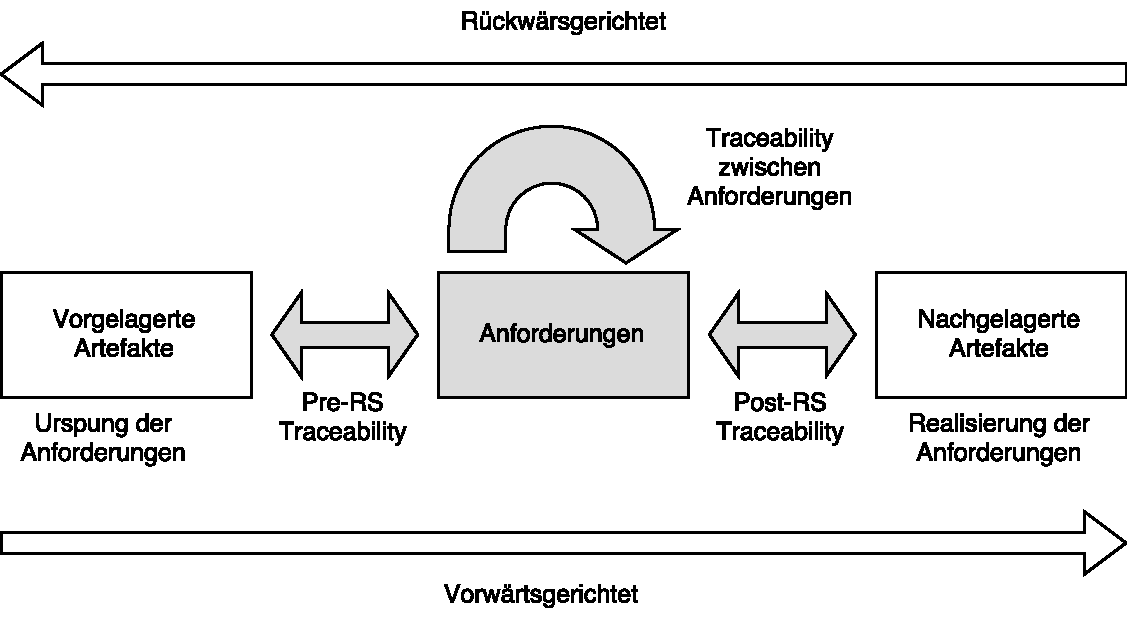
\includegraphics[width=3.4in]{PohlRupp2015_Fig_8_5.pdf}
  \caption{nach \cite[Fig. 8.5]{Pohl2015BasiswissenIREB-Standard}}
  \label{fig:abb1}
\end{figure}

Wie in \ref{fig:abb1} dargestellt wird zwischen drei Arten von Verfolgbarkeit unterschieden:

\begin{itemize}
    \item \textbf{Pre-RS:} Alle Beziehungen zu Artefakten die einer Anforderung vorgelagert sind z.B. Dokumente, Interviews etc. Im allgemeinen der Ursprung einer Anforderung
    \item \textbf{Post-RS:} Alle Beziehungen die einer Anforderung nachgelagert sind z.B Implementierung, Tests. Im allgemeinen die Auswirkung einer Anforderung
    \item \textbf{Verfolgbarkeit zwischen Anforderungen:} Abhängigkeiten oder Beziehungen zwischen Anforderungen. So kann z.B. eine Anforderung aus einem Konflikt zwischen zwei Anforderungen entstehen oder diese ersetzen. Im allgemeinen spricht man von einer Verfolgbarkeit über die Spezifikation \cite{Pohl2015BasiswissenIREB-Standard}.
\end{itemize}

Auf dem Pre-RS \& Post-RS Modell aufbauend, führt Pohl eine weitere Differenzierung ein, wie in \ref{fig:abb2} dargestellt.

\begin{figure}[!htb]
  \centering
  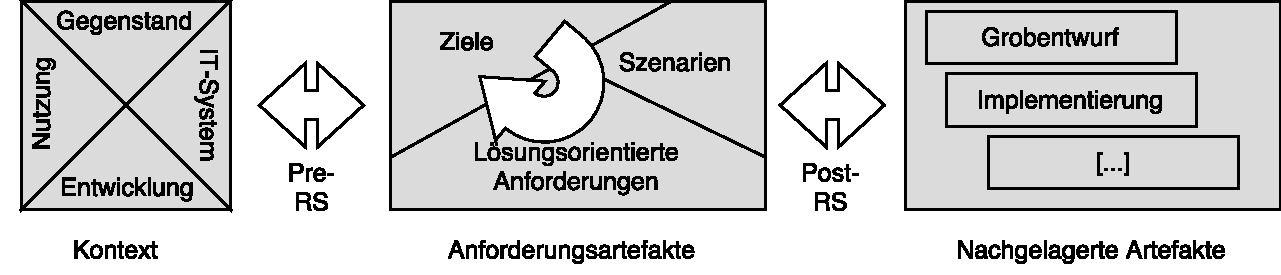
\includegraphics[width=3.4in]{Pohl2008_Fig_30_3.pdf}
  \caption{nach \cite[Fig. 30.3]{Pohl2008RequirementsTechniken}}
  \label{fig:abb2}
\end{figure}

Die \enquote{Erweiterte Pre- und Post-Traceability} präzisiert die Sicht auf die vor- und nach-gelagerten Artefakte. Die Pre-RS Traceability beschreibt alle Beziehungen zwischen Anforderungsartefakten und Aspekten in einer der 4 Sichten des Systemkontext. Die Post-RS Traceability beschreibt alle Beziehungen zwischen Anforderungsartefakten und nachgelagerten Artefakten die im Entwicklungsprozess entstehen. Die Beziehung zwischen Anforderungen umfasst zusätzlich die Verfolgbarkeit zwischen Zielen, Szenarien und lösungsorientierten Anforderungen \cite{Pohl2008RequirementsTechniken}.

Zusammenfassend lässt sich festhalten, das Requirements Traceability die Verfolgbarkeit einer Anforderung vom Ursprung bis zur Implementierung beschreibt. Diese Beziehung muss bidirektional sein, d.h. sie ist in vorwärts- wie in rückwärtsgerichteter Richtung möglich. Eine Verfolgbarkeit besteht dabei zwischen allen vor- und nach-gelagerten Artefakten im Entwicklungsprozess, wobei nach Pohl diese aus dem Kontext, Anforderungsartefakten und nachgelagerten Entwicklungsartefakten besteht. Die Qualität einer Verfolgbarkeit ist bestimmt durch die Vollständigkeit, Konsistenz und Fehlerfreiheit der Verfolgbarkeitsinformationen.

Die Erfassung ist jedoch ein manueller Prozess und dadurch fehleranfällig. Nach Walia \& Carver ist eine der Ursachen für Probleme im Requirements Engineering auf Inkonsistenzen in der Requirements Traceability zurückzuführen, die mitunter durch ein unzureichendes Requirements Management oder durch Fehler von Teammitgliedern verursacht werden \cite{Walia2009AErrors}. 

Um die Qualität sicherzustellen ist es wichtig zu wissen welche Probleme in der Requirements Tracebility existieren und welche Methoden es gibt um diese zu vermeiden.
Das können präventive sowie kurative Maßnahmen sein.

Als zentrales Ziel dieses Systematic Literature Review steht somit die

\enquote{Identifikation von Qualitätsproblemen in der Requirements Traceability, um sie frühzeitig erkennen und vermeiden zu können.

%In diesem Systematic Literature Review soll daher der aktuelle Forschungsstand zu Problemen im Management von Requirements Traceability und Maßnahmen ihrer Vermeidung näher beleuchtet werden.

%\section{Vorgehen}
%Zu Beginn wurde ein Systematic Literature Review (SLR) durchgeführt, um Probleme im Management von Requirements Traceability zu bestimmen, die die Qualität negativ beeinflussen. 
\section{Forschungsmethode}
\label{sec:Forschungsmethode}
Den Richtlinien in \cite{Keele2007GuidelinesEngineering} folgend, wurde ein Systematisches Literatur Review (SLR) nach Kitchenham et al. durchgeführt. Das Dokument folgt dem Aufbau in \cite{Walia2009AErrors} und umfasst die folgenden Schritte 

\begin{itemize}
    \item Formulierung eines Review-Protokolls
    \item Durchführen des Reviews
        \begin{itemize}
            \item Identifizierung von Primärstudien
            \item Evaluierung \& Auswahl
            \item Datenextraktion
            \item Datensynthese
        \end{itemize}
    \item Analyse der Ergebnisse
    \item Auswertung der Ergebnisse
    \item Diskussion der Ergebnisse
\end{itemize}

Ein Review Protokoll enthält alle Forschungsfragen, Methoden, Vorgehensweisen etc. die benötigt werden um ein SLR durchführen zu können Es wird im Vorfeld des Reviews angefertigt, um zu vermeiden, dass das Review durch die Erwartungshaltung des Forschers getrieben wird und damit an Objektivität verliert (Reseracher bias). Nach Durchführung des Reviews wird aus den Ergebnissen der Datensynthese eine Analyse und Auswertung der Ergebnisse durchgeführt um die gestellten Forschungsfragen beantworten zu können \cite{Walia2009AErrors}.

\subsection{Forschungsfragen}

Das zentrale Ziel dieses SLR war es, Qualitätsprobleme im Management der Requirements Traceability und mögliche Lösungsanasätze zu identifizieren und zu klassifizieren. Die zugehörige Fragestellung für den Review war also

\enquote{Welche Arten von Qualitätsprobleme existieren im Management der Requiremenst Traceability und wie können diese behoben werden?}

Zur Beantwortung der Fragestellung, war es notwendig entsprechende Forschungsfragen zu definieren, die sich auf die Beantwortung dieser Fragestellung fokussierten und damit im Review auch zu verwertbaren Ergebnissen führten. Nach einer ersten Analyse des Forschungsgebietes, konnte festgestellt werden, dass ein Teil der Forschungsarbeiten sich nur indirekt auf Qualitätsprobleme im Management von Requirements Traceability bezogen. Im Fall, dass ein Lösungsansatz zur Thematik genannt worden ist, war dieser nicht zwingend nur für den speziellen Anwendungsfall einsetzbar.

Aus den Ergebnissen der Analyse konnte eine Vorgehensweise identifiziert werden, die die Beobachtungen wiederspiegelte und im Einklang mit den Forschungsfragen dieses Reviews stand. Die Abbildung \ref{fig:abb_forschungsfragen} zeigt das Ergebnis der ersten Analysephase und damit die Festlegung der Vorgehensweise für den weiteren Reviewverlauf

\begin{figure}[!htb]
  \centering
  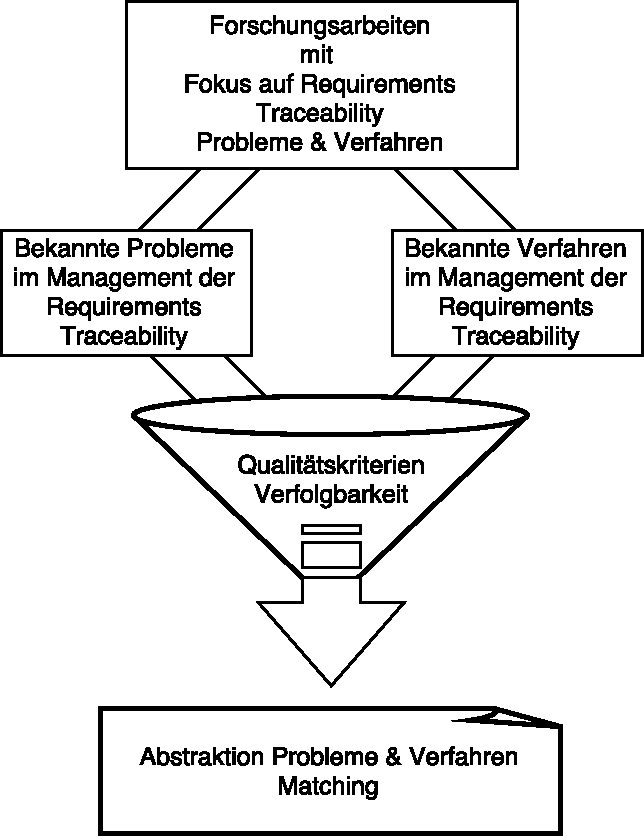
\includegraphics[width=2in]{forschungsfragen_diagramm_v2.pdf}
  \caption{Vorgehensweise zur Beantwortung der Forschungsfragen}
  \label{fig:abb_forschungsfragen}
\end{figure}

% Ggf. anhand des Forschungsziels nochmal zu präzisieren!
Wie in \ref{fig:abb_forschungsfragen} dargestellt wurde das Vorgehen in mehrere Etappen eingeteilt. Im ersten Schritt stand die Identifikation von Forschungsarbeiten die im Themengebiet Requirements Traceability angesiedelt waren und sich mit Problemen oder Lösungsansätzen in diesem Bereich beschäftigten. Entsprechend mussten die Forschungsfragen und Auswahlkriterien so formuliert werden, dass die entsprechenden Arbeiten erfasst wurden. Anhand der Analyse wurde sich dazu entschieden, im weiteren Verlauf Probleme und Verfahren zu separieren und in Bezug zu den Qualitätskriterien zu stellen, da nach den Ergebnissen aus der Analyse nicht jeder Lösungsansatz auf einen Anwendungsfall beschränkt war. Im letzten Schritt folgte dann eine Zusammenführung aller Daten um die Abdeckung von Problemen und Verfahren zu bestimmen um die zentrale Forschungsfrage beantworten zu können.

Die Tabelle \ref{tab:forschungsfragen} zeigt die Forschungsfragen, die aus der Vorgehensweise und der zentralen Fragestellung für diesen Review extrahiert wurden. Um Willkür zu vermeiden, wurde in Tabelle \ref{tab:motivationen} zu jeder Frage eine Motivation niedergeschrieben, die die Sinnhaftigkeit einer Frage separat darstellt. Die erste Frage befasst sich mit möglichen Qualitätsproblemen im Management der Requirements Traceability mit dem Ziel, diese möglichst vollständig zu erfassen. Die zweite Frage befasst sich separat mit den Verfahren zu Behandlung von Qualitätsproblemen und Hinweisen dazu in den erfassten Forschungsarbeiten. Die dritte und letzte Frage fasst die gesammelten Daten zu abstrakteren Vorgehensweisen zusammen, anhand derer ein Abdeckungsgrad für klassifizierte Qualitätsprobleme bestimmt werden kann. Die Fragen 1 und 2 erforderten einen systematische Literaturreview.

% ------------------------------------------------------------------------------------------
% --- FORSCHUNGSFRAGEN + MOTIVATIONE

\begin{table*}[t]
\renewcommand{\arraystretch}{1.3}
\centering
\begin{tabularx}{\textwidth}{@{}X@{}}
\toprule
Forschungsfragen \\ \midrule
1. Welche Arten von Qualitätsproblemen können während des Softwarelebenszyklus im Management der Requirements Traceability entstehen? \\
\hspace*{10mm}1.1 Welche Arten von Qualitätsproblemen in der Requirements Traceability wurden in der vorhandenen Literatur identifiziert? \\
\hspace*{10mm}1.2 Welche Qualitätsprobleme können durch die Analyse ihrer Ursache identifiziert werden? \\
\hspace*{10mm}1.3 Beeinflussen die gefundenen Probleme die Kriterien in \ref{tab:qualitaet_verfolgbarkeit}? \\
2. Welche Verfahren existieren im Management der Requirements Traceability zur Behandlung von Qualitätsproblemen? \\
\hspace*{10mm}2.1 Greift die Literatur Prozesse oder Methodiken auf, die zu einer Verbesserung der Qualität beitragen? \\
\hspace*{10mm}2.2 Addressieren die gefundenen Verfahren die Kriterien in \ref{tab:qualitaet_verfolgbarkeit}? \\
3. Lassen sich die Erkenntnisse aus 1-2 zu Aussagen über mögliche Verfahrensweisen im spezifischen Anwendungsfall zusammenfassen? \\
\bottomrule
\end{tabularx}
\caption{Definierte Forschungsfragen}
\label{tab:forschungsfragen}
\end{table*}

\begin{table*}[t]
    \centering
    \begin{tabularx}{\textwidth}{X}
        \toprule
        Motivationen \\ \midrule
        1. Unabhängige Erfassung aller Qualitätsprobleme die mindestens eine der Kriterien für Qualität von Verfolgbarkeit beinflussen \\
        2. Unabhängige Erfassung aller Verfahren die mindestens einer der Kriterien für Qualität von Verfolgbarkeit beeinflussen \\
        3. Bestimmen von Verfahren und ihrer Abdeckung für die Behandlung von Qualitätsproblemen \\
    \bottomrule
    \end{tabularx}
    \caption{Motivationen zu den gestellten Forschungsfragen in \ref{tab:forschungsfragen}}
    \label{tab:motivationen}
\end{table*}

% ------------------------------------------------------------------------------------------

\subsection{Quellenauswahl und Suche}
\label{subsec:Quellenauswahl}

Die initiale Auswahl der Quellen erfolgte anhand der unten beschriebenen Auswahlkriterien:

\begin{itemize}
    \item Es wurde nach Datenbanken gesucht, die:
        \begin{itemize}
            \item Veröffentlichungen aus Zeitschriften oder Konferenzen über Software Engineering oder Software Qualität enthielten
            \item Eine Suchmaschine mit erweitertem Suchmechanismus offerierten. Der Suchmechanismus musste die Expertensuche nach einer Folge von logischen Ausdrücken unterstützen
            \item Das Volltextdokument musste über die Datenbank oder andere Hilfsmittel abrufbar sein
        \end{itemize}
    \item Die gefundenen Datenbanken wurden auf ein minimales Set reduziert um die Anzahl redundanter Papiere minimal zu halten
    \item Andere Quellen wurden hinzugefügt, die nach Einschätzung des Forschers eine Relevanz zum Thema haben
\end{itemize}

Eine Einschränkung der Datenbanken auf Zeitschriften und Konferenzen im Bereich Software Engineering oder Software Qualität ergab sich aus der initialen Analyse unter der Berücksichtigung, dass das Management der Requirements Traceability teil des Requirements Engineering im Software Engineering ist. Da der Fokus dieser Arbeit auf Qualität lag, wurde sich letztendlich für die oben genannten Bereiche entschieden um den Suchraum möglichst weit zu fassen. Der erweiterte Suchmechanismus nach logischen Ausdrücken war Vorraussetzung für die geplante Suche nach Suchstrings auf die in diesem Kapitel noch näher eingangen wird. Neben den klassischen Datenbanken war es nach der Auffassung des Forschers notwendig, weitere Quellen wie Buchquellen zu betrachten um die Vollständigkeit des Reviews sicherzustellen. Da Forschungspapiere in mehreren Datenbanken auftauchen konnten und dies einen erheblichen Mehraufwand bedeutet hätte, wurden die gefundenen Datenbanken auf ein minimales Set reduziert um die Anzahl redundanter Papiere zu minimieren. Tabelle \ref{tab:quellen_review} zeigt das Ergebnis der Quellenauswahl

\begin{table}[!ht]
\renewcommand{\arraystretch}{1.3}
\centering
\begin{threeparttable}
\begin{tabularx}{\columnwidth}{@{}lX@{}}
\toprule
Kriterium & Auswirkung \\ \midrule
Datenbanken & ACM Digital Library, IEEE Xplore, Science Direct (Elsevier), SpringerLink \\
Andere Artikel & SWEBOK - Software Engineering Body of Knowlege \\
Erweiterte Quellen & Buchquellen \\
\bottomrule
\end{tabularx}
\medskip
      %\footnotesize\textbf{Legende:}\smallskip
      %\begin{tablenotes}\footnotesize
      %\item[*] In \cite{Kollanus2010Test-DrivenApproach} werden die gleichen Studien wie in \cite{Kollanus2011CriticalDevelopment} untersucht.
      %\end{tablenotes}
\end{threeparttable}
\caption{Quellen für den Review}
\label{tab:quellen_review}
\end{table}

Um die Datenbanken zu durchsuchen, wurden aus den zu reviewenden Forschungsfragen 1-2 übergeordnete Suchbegriffe in englischer Sprache abgeleitet. Diese wurden dann mit Synonymen, Abkürzungen und alternativen Schreibweisen aus den in der Analyse gefundenen Büchern, Papieren etc. angereichtert um eine weite Abdeckung des Suchbegriffes sicherzustellen. Da aus der Analyse hervorging, dass Lösungsansätze und Probleme üblicherweise im selben Dokument genannt werden, wurde sich für die Konstruktion eines globalen Suchstrings entschieden, dessen Ergebnisse dann für den Review beider Forschungsfragen verwendet worden sind. Im Folgenden der globale Suchstring der für die Suche in den Datenbanken verwendet worden ist

\enquote{((requirements traceability OR traceability) AND (quality OR condition OR character OR property OR attribute OR aspect) AND (problem OR error OR mistake OR reason OR fault OR defect OR inconsistent OR incomplete OR flaw OR lapse OR slip OR err) AND ((abstraction OR root cause OR cause OR origin OR element OR source) OR (improvement OR method OR technique OR approach OR mechanism OR process OR taxonomy) OR (identify OR analyze OR classify) OR (recovery OR reconstruction OR restoration OR recall) OR (correction OR adjustment OR improvement OR amelioration)))}

Wenn sinnvoll, wurden die Filterkriterien dem Fokus des Reviews angepasst und in der Durchführung dokumentiert. Die Auswahl der gefundenen Papiere erfolgte dann in einem mehrstufigen Selektionsprozess. Er umfasste die folgenden Schritte

\begin{enumerate}
    \item Lesen des Titels um Papiere auszuschließen, die keinen klaren Bezug zum Thema haben
    \item Lesen des Abstracts um Papiere weiter anhand ihres Bezugs zum Thema einzugrenzen
    \item Prüfen der Papiere auf die definierten Inklusions- und Exklusionskriterien in \ref{tab:inklusions_exklusionkriterien} um den Bezug zum Thema klar herauszustellen
    \item Prüfen der Papiere auf die definierten Qualitätskriterien in Tabelle \ref{tab:qualitaetskriterien_review} um die Qualität der Forschungsarbeit sicherzustellen
\end{enumerate}

Bei der Durchführung des Reviews musste eine zusätzliche Rahmenbedingung neben dem Selektionsprozess eingeführt werden. Beim Durchsuchen der ersten Datenbank "Science Direct (Elsevier)" wurde das Limit der Anzeige von Suchergebnisse erreicht (1000). Beim Review der bisher gesammelten Treffer konnte zudem festgestellt werden, dass die Trefferquote nach den ersten Seiten dramatisch sank. Daher wurde auf Grund der Limitierung, der durchschnittlichen Anzahl an Treffer pro Datenbank (> 2000) sowie der stark sinkenden Trefferquote das Limit für die Suche in einer Datenbank auf die ersten 10 Ergebnisseiten limitiert.

Für den Review galt es noch die Inklusions- und Exklusionskriterien, sowie Qualitätskriterien für die finale Auswahl von Forschungspapieren zu definieren. Tabelle \ref{tab:inklusions_exklusionkriterien} zeigt die Inklusions- und Exklusionkriterien wie sie für den Review angewendet wurden.

\begin{table}[!ht]
\renewcommand{\arraystretch}{1.3}
\centering
\begin{threeparttable}
\begin{tabularx}{\columnwidth}{@{}XX@{}}
\toprule
Inklusionskriterien & Exklusionskriterien \\ \midrule
Forschungsarbeit beschäftigt sich mit Problemen in der Requirements Traceability & Forschungsarbeit hat keinen Bezug zum Forschungsgebiet \\
Forschungsarbeit beschäftigt sich mit Ursachen für Problemen in der Requirements Traceability & Forschungsarbeit hat keinen Bezug zu den gestellten Forschungsfragen \\
Forschungsarbeit beschäftigt sich mit Methodiken im Management der Requirements Traceability & Forschungsarbeit ist nicht auf Englisch \\
Empirische Studie (qualitative und quantitative) über Praktiken im Management von Requirements Traceability & Ergebnisse einer Forschungsarbeit sind unklar oder mehrdeutig \\
\bottomrule
\end{tabularx}
\medskip
      %\footnotesize\textbf{Legende:}\smallskip
      %\begin{tablenotes}\footnotesize
      %\item[*] In \cite{Kollanus2010Test-DrivenApproach} werden die gleichen Studien wie in \cite{Kollanus2011CriticalDevelopment} untersucht.
      %\end{tablenotes}
\end{threeparttable}
\caption{Inklusions- und Exklusionkriterien}
\label{tab:inklusions_exklusionkriterien}
\end{table}

Die Inklusionskriterien wurden so gewählt, dass sie den Themenbezug zur Requirements Traceability und den Forschungsfragen herausstellten. Die Exklusionskriterien grenzten dies weiter ab. Zusätzlich wurden direkte Ausschlusskriterien eingefügt ohne die eine Forschungsarbeit nicht verwertbar gewesen wäre. Als letzte Instanz für die Auswahl standen die Qualitätskriterien in Tabelle \ref{tab:qualitaetskriterien_review}.

\begin{table}[!ht]
\renewcommand{\arraystretch}{1.3}
\centering
\begin{threeparttable}
\begin{tabularx}{\columnwidth}{@{}XX@{}}
\toprule
Qualitätskriterien \\ \midrule
Basiert die Studie auf sinnvollen Annahmen? \\
Ist die Vorgehensweise angemessen? \\
Werden in der Studie Maßnahmen angewendet, um Mehrdeutigkeiten zu vermeiden? \\
Kann die Studie nachvollzogen werden? \\
\bottomrule
\end{tabularx}
\medskip
      %\footnotesize\textbf{Legende:}\smallskip
      %\begin{tablenotes}\footnotesize
      %\item[*] In \cite{Kollanus2010Test-DrivenApproach} werden die gleichen Studien wie in \cite{Kollanus2011CriticalDevelopment} untersucht.
      %\end{tablenotes}
\end{threeparttable}
\caption{Qualitätskriterien}
\label{tab:qualitaetskriterien_review}
\end{table}

Ihre Aufgabe bestand in der Qualitätssicherung um nur Forschungsarbeiten in die finale Liste aufzunehmen, die den Mindestanforderungen an die Qualität genügten.

\subsection{Durchführung}

Von den 4 identifizierten Datenbanken konnten nur 3 durchsucht werden, da die IEEXplore Datenbank zwar den Kriterien für die Auswahl von Datenbanken entsprach, aber ein Limit von 15 Schlüsselwörtern für logische Ausdrücke hatte. Die Anwendung des globalen Suchstrings war daher nicht möglich. 

Die Suche in den verbleibenden 3 Datenbanken ergab über 10000 Treffer wobei 60\% davon in der ACM Digital Library gefunden wurden. Den festgelegten Rahmenbedingungen im Selektionsprozess folgend, wurden nur jeweils die ersten 10 Ergebnisseiten anhand der Selektionskriterien bewertet. Insgesamt sind 650 Papiere bewertet worden, davon wurden 92 anhand ihres Titels ausgewählt. Nach Lesen des Abstracts blieben noch 35 Forschungsarbeiten übrig, von denen 14 nach Lesen des Volltextes den festgelegten Inklusions- und Exklusionskriterien genügten. Erfreulicherweise waren alle ausgewählten Forschungsarbeiten von hoher Qualität und entsprachen den Qualitätskriterien.

In Tabelle \ref{tab:quellenauswahl_quote} sind die Ergebnisse des Reviews nochmal aufgesplittet. Anhand der Ergebnisse kann festgehalten werden, das die initiale Trefferquote mit \~15\% über den Erwartungen lag und obwohl in der Datenbank ScienceDirect 50 Forschungsarbeiten mehr durchsucht wurden, die Quote nur marginal höher war. Das ist ein gutes Indiz für die Korrektheit der Annahme das die Trefferquote in späteren Ergebnisseiten signifikant sinkt. Außerdem war keiner der ausgewählten Forschungsarbeiten redundant was für die Auswahlkriterien der Quellen sprach. Einzig die Trefferquote für die Datenbank ACM Digital Library lag, trotz der höheren Trefferanzahl weit unter dem Mittel der anderen beiden Datenbanken SpringerLink und ScienceDirect (Elsevier). Um Fehler bei der Suche auszuschließen wurde nochmal die gleiche Suche mit weiter einschränkenden Filtern durchgeführt. Die Trefferanzahl ließ sich aber nicht signifikant verringern um einen erneuten Review zu rechtfertigen. Es kann daher nur angenommen werden, dass ein oder mehrere Faktoren wie die Menge an verfügbaren Dokumenten, die schiere Anzahl an Ergebnissen oder der Suchalgorithmus für die Auswertung von logischen Ausdrücken hier zu den schlechteren Ergebnissen geführt haben könnten.

% Noch einfügen? Je nach Ergebnisse der Extraktion und Analyse zu erwägen
%Von den 14 ausgewählten Forschungsarbeiten waren 3 dem Forscher bereits aus der Analyse bekannt \cite{Mder2012TowardsMaintenance, Hu2016DetectionTaxonomy, Merten2016DoData}. Einige relevante Arbeiten wurden dabei nicht erfasst und mussten separat hinz

\begin{table}[!ht]
\renewcommand{\arraystretch}{1.3}
\centering
\begin{threeparttable}
\begin{tabularx}{\columnwidth}{@{}lXXrXXX@{}}
\toprule
Datenbank & Anz. Papiere & Nach Titel & Quote & Nach Abstract & Nach Inkl.-Exkl. & Nach Qualität \\ \midrule
ScienceDirect & 250 & 42 & 16.8 \% & 17 & 7 & 7 \\
SpringerLink & 200 &  38 & 19 \% & 15 & 6 & 6 \\
ACM & 200 & 12 & 6 \% & 3 & 1 & 1 \\
\bottomrule
\end{tabularx}
\medskip
      %\footnotesize\textbf{Legende:}\smallskip
      %\begin{tablenotes}\footnotesize
      %\item[*] In \cite{Kollanus2010Test-DrivenApproach} werden die gleichen Studien wie in \cite{Kollanus2011CriticalDevelopment} untersucht.
      %\end{tablenotes}
\end{threeparttable}
\caption{Zusammenfassung Ergebnisse Review}
\label{tab:quellenauswahl_quote}
\end{table}

\subsection{Datenextraktion und Datensynthese}

Für die Datenextraktion wurde im Vorfeld des Reviews ein Datenextraktionsformular entwickelt. Der Einsatz solcher Formulare ist üblich in systematischen Literraturreviews um die gesammelten Informationen der Extraktion präzise und konsistent dokumentieren zu können. Das Ziel einer Datenextraktion ist die vollständige Erfassung aller relevanten Informationen, um die gestellten Forschungsfragen beantworten zu können. Ein Datenextraktionsformular wird im Vorfeld entwickelt und enthält alle Datenelemente die relevant sind für die Extraktion.

% Noch zu überarbeiten!
%Für diesen Review wurden zwei Datenextraktionsformulare entwickelt. Ein Formular enthält die Grunddaten die generell erfasst werden müssen. Das zweite Formular erfasst die Probleme und Lösungsansätze.

\begin{table}[!ht]
\renewcommand{\arraystretch}{1.3}
\centering
\begin{threeparttable}
\begin{tabularx}{\columnwidth}{@{}sm@{}}
\toprule
Datenelement & Beschreibung  \\ \midrule
Identifier & Katalog Identifikationsnummer (DOI) \\
Bibiliographie & Author, Titel, Jahr, Quelle \\
Typ & Book section, Conference proceeding, Journal \\
\bottomrule
\end{tabularx}
\medskip
      %\footnotesize\textbf{Legende:}\smallskip
      %\begin{tablenotes}\footnotesize
      %\item[*] In \cite{Kollanus2010Test-DrivenApproach} werden die gleichen Studien wie in \cite{Kollanus2011CriticalDevelopment} untersucht.
      %\end{tablenotes}
\end{threeparttable}
\caption{Daten die aus allen Papieren extrahiert worden sind}
\label{tab:dataextraction_general}
\end{table}

\begin{table*}[!ht]
    \centering
    \begin{tabularx}{\textwidth}{ssX}
        \toprule
        Fokus & Datenelement & Beschreibung \\ \midrule
       Probleme im Management der Requirements Traceability & Problem & Kurze Beschreibung des allgemeinen Problems \\
        & Kontext & In welchem Kontext entsteht es? \\
        & Phase & Welche Phase der Requirements Traceability betrifft das Problem? \\
        & Ursache & Welche Ursache hat es?  \\
        & Auswirkung  & Welche Auswirkungen hat es im Bezug auf die Qualität von Verfolgbarkeit? \\
        Verfahren zur Behandlung von Qualitätsproblemen & Lösungsansatz & Kurze Beschreibung des Lösungsansatzes \\
        & Fachgebiet  & Gebiet in dem der Ansatz angesiedelt ist  \\
        & Art & Art des Ansatzes : Manuell, Semi-Automatisch, Automatisch \\
        & Unterstützung & Welche Aspekte unterstützt das Verfahren? \\
        & Vorgehen & Beschreibung der Verwendung, Ablauf etc. \\
        & Nutzen & Welcher Nutzen kann aus der Verwendung des Verfahrens gezogen werden? \\
        & Limitierungen & Wo liegen die Grenzen des Verfahrens? \\
    \bottomrule
    \end{tabularx}
    \caption{Daten die für das jeweilige Forschungsziel extrahiert worden sind}
    \label{tab:dataextraction_special}
\end{table*}



\section{Auswertung des Reviews}
\label{sec:AuswertungReview}

\subsection{Frage 1: Welche Arten von Qualitätsproblemen können während des Softwarelebenszyklus im Management der Requirements Traceability entstehen?}

Aus den 14 ausgewählten Forschungsliteraturen ging hervor, dass alle aktuelle relevanten Qualitätsprobleme sich auf den Kontext von großen Softwaresystemen bezogen. Die Größe und Komplexität kann dort, ohne adequates Management der Requirements Traceability großen Einfluss auf das Projekt bis hin zum gesamten Projekterfolg haben. Als ein weiterer Faktor kann die sich ändernde Projektumgebung genannt werden, die die Notwendigkeit von Verfolgbarkeit weiter in den Vordergrund gerückt hat.

Die Erkenntnisse zeigen, das die Etablierung von Verfolgbarkeit weniger ein Thema ist als ihr direkter Verfall durch Evolution des Softwaresystems. Ein weiterer Punkt steht in der Wiederherstellung der Qualität der Verfolgbarkeit. Beide Qualitätsprobleme erzeugen hohe Aufwände und Kosten und stehen entgegen dem Nutzen und den Motivationen der eigentlichen Einführung von Verfolgbarkeit. In Bezug zu den identifizierten Motivationen stehen die zentralen Aspekte das Änderungsmanagement durch Evolution, die Qualitätssicherung und Wartbarkeit wie auch die Nachweisbarkeit \& Akzeptanz einzelner Systemfunktionen.

\subsection{Frage 1.1: Welche Arten von Qualitätsproblemen in der Requirements Traceability wurden in der vorhandenen Literatur identifiziert?}

Entgegen den Erwartungen ähnelten sich die Problemstellungen in den 14 ausgewählten Literaturen. Daher wurden diese in der Tabelle \ref{tab:auswertung_probleme_allgemein} zu zwei zentralen Problemen im Management der Requirements Traceability zusammengefasst.

\begin{table}[!ht]
\renewcommand{\arraystretch}{1.3}
\caption{Probleme in der Requirements Traceability}
\label{tab:auswertung_probleme_allgemein}
\centering
\begin{tabularx}{\columnwidth}{@{}sm@{}}
\toprule
1. Evolution von Softwaresystemen & \cite{Saputri2016EnsuringApproach,Bavota2014EnhancingInformation,Spanoudakis2004Rule-basedRelations,Javed2014ACode,Tsuchiya2015InteractiveLogs,Omoronyia2011ExploringTraceability,Lago2009AManagement, Mader2009EnablingRelations,Mder2012TowardsMaintenance,Ghabi2015ExploitingCode} \\
2. Wiederherstellung von Verfolgbarkeit in bestehenden Softwaresystemen & \cite{Mder2007CustomizingProcess,Leuser2010TacklingSpecifications,Merten2016DoData} \\
\bottomrule
\end{tabularx} 
\end{table}

Interessanterweise deckten sich die identifizierten Probleme im Management mit den Erkenntnissen von Walia \& Carver \cite{Walia2009AErrors}, die in ihrer Forschungsarbeit anhand eines SLRs herausgefunden hatten, dass die häufigsten Fehler im Requirements Management auf Grund von

\begin{enumerate}
    \item Inadequatem Änderungsmanagement, eingeschlossen der Analyse der Auswirkung durch Ändern von Anforderungen
    \item Inadequater/Schlechter Requirements Traceability
\end{enumerate}

entstehen. \cite{Walia2009AErrors}

Entsprechende Ursachen zu den Probleme wurden in der Literatur implizit oder explizit genannt, siehe Tabelle \ref{tab:auswertung_probleme_ursachen}.

\begin{table}[!ht]
\renewcommand{\arraystretch}{1.3}
\caption{Ursachen für Probleme}
\label{tab:auswertung_probleme_ursachen}
\centering
\begin{tabularx}{\columnwidth}{@{}mss@{}}
\toprule
Fehlen adequater Toolunterstützung & \cite{Saputri2016EnsuringApproach, Mder2007CustomizingProcess, Spanoudakis2004Rule-basedRelations, Ghabi2015ExploitingCode, Leuser2010TacklingSpecifications, Omoronyia2011ExploringTraceability, Tsuchiya2015InteractiveLogs} \\
Aufwand nicht im Verhältnis zum Nutzen & \cite{Javed2014ACode,Lago2009AManagement,Spanoudakis2004Rule-basedRelations, Omoronyia2011ExploringTraceability, Bavota2014EnhancingInformation, Saputri2016EnsuringApproach, Mder2012TowardsMaintenance, Mader2009EnablingRelations} \\
Fehleinschätzung der Notwendigkeit & \cite{Leuser2010TacklingSpecifications, Ghabi2015ExploitingCode}
Einsatz inadequater Tools & \cite{Merten2016DoData} \\
\bottomrule
\end{tabularx}
\end{table}

Als zentrale Ursache für eine schlechte Qualität im Management der Requirements Traceability wird in 7 Literaturen das \enquote{Fehlen adequater Tooluntersützung} genannt. Entsprechend kann angenommen werden das auf Grund dieses Umstands eine vollständige Erfassung so wahrgenommen wird als stände ihr \enquote{Aufwand nicht im Verhältnis zum Nutzen}.

Aus den zentralen Problemen und Ursachen lassen sich erste Aussagen über Qualitätsprobleme im Management der Verfolgbarkeit ableiten

\begin{itemize}
    \item Fehlen adequater Mechanismen um den Verfall von Verfolgbarkeit durch Evolution zu verhindern
    \item Fehlen adequater Mechanismen um die Qualität von Verfolgbarkeit in bestehenden Spezifikationen wiederherzustellen
\end{itemize}

\subsection{Frage 1.2: Welche Qualitätsprobleme können durch die Analyse ihrer Ursache identifiziert werden?}

Alle Probleme wurden explizit oder implizit im Kontext von großen Softwareprojekten genannt. Die Notwendigkeit von Traceability ergibt sich dort auf Grund der Größe oder Komplexität eines Softwareprojekts und ihres Einflusses auf den Projekterfolg \cite{Lago2009AManagement, Mder2007CustomizingProcess, Leuser2010TacklingSpecifications, Tsuchiya2013RecoveringProducts, Ghabi2015ExploitingCode}. Als zusätzlicher Faktor für die Notwendigkeit spricht eine Veränderung der Anforderungen an die Entwicklung von Softwaresystemen, siehe Tabelle \ref{tab:auswertung_probleme_ursachen_needs}.

\begin{table}[!ht]
\renewcommand{\arraystretch}{1.3}
\caption{Veränderungen in den Projektgegebenheiten}
\label{tab:auswertung_probleme_ursachen_needs}
\centering
\begin{tabularx}{\columnwidth}{@{}ms@{}}
\toprule
Fortschritte in den verfügbaren Technologien & \cite{Saputri2016EnsuringApproach} \\
Höhere Nutzererwartungen & \cite{Saputri2016EnsuringApproach} \\
Evolutionäre Entwicklung von Softwaresystemen & \cite{Saputri2016EnsuringApproach} \\
Häufige Veränderungen in den Anforderungen & \cite{Mder2007CustomizingProcess} \\
Notwendigkeit für sicherheitsrelevante Systeme & \cite{Leuser2010TacklingSpecifications} \\
Implizite Notwendigkeit für die Wartbarkeit eines Systems & \cite{Lago2009AManagement} \\
\bottomrule
\end{tabularx} 
\end{table}

Aus der Extraktion von Motivationen für den Einsatz von Verfolgbarkeit ergaben sich ähnliche Gründe die einen Bezug zu den Veränderungen in Tabelle \ref{tab:auswertung_probleme_ursachen_needs} hatten. Tabelle \ref{tab:auswertung_probleme_ursachen_motivation} zeigt das Ergebnis der Extraktion. Da die Definitionen teils implizit oder natürlichsprachlich waren, wurden die Intentionen den Begrifflichkeiten und Definitionen nach dem Standardkwerk von Pohl \cite[Tab. 30-1]{Pohl2008RequirementsTechniken} zugeordnet.

\begin{table}[!ht]
\renewcommand{\arraystretch}{1.3}
\caption{Motivationen für Probleme}
\label{tab:auswertung_probleme_ursachen_motivation}
\centering
\begin{tabularx}{\columnwidth}{@{}ms@{}}
\toprule
Änderungsmanagement & \cite{Spanoudakis2004Rule-basedRelations, Javed2014ACode, Tsuchiya2013RecoveringProducts, Saputri2016EnsuringApproach, Omoronyia2011ExploringTraceability,Bavota2014EnhancingInformation, Mder2007CustomizingProcess, Mader2009EnablingRelationss, Mder2012TowardsMaintenance, Ghabi2015ExploitingCode} \\
Nachweisbarkeit \& Akzeptanz & \cite{Spanoudakis2004Rule-basedRelations, Bavota2014EnhancingInformation, Leuser2010TacklingSpecifications} \\
Qualitätssicherung, Wartung und Pflege & \cite{Spanoudakis2004Rule-basedRelations, Javed2014ACode, Tsuchiya2013RecoveringProducts, Saputri2016EnsuringApproach, Bavota2014EnhancingInformation, Mder2007CustomizingProcess, Mader2012TowardsMaintenance, Lago2009AManagement} \\
\bottomrule
\end{tabularx} 
\end{table}

Anhand der Erkenntnisse zu Veränderungen in Tabelle \ref{tab:auswertung_probleme_ursachen_needs}, Motivationen in Tabelle \ref{tab:auswertung_probleme_ursachen_motivation} sowie bekannten Ursachen aus Tabelle \ref{tab:auswertung_probleme_ursachen} konnte auf die bereits identifizierten Qualitätsprobleme ein Rückgeschlossen hergestellt werden. Weitere Qualitätsprobleme wurden nicht identifiziert.

\subsection{Frage 1.3: Beeinflussen die gefundenen Probleme die Kriterien in \ref{tab:qualitaet_verfolgbarkeit}?}

Alle identifizierten Probleme beeinflussen mindestens eine der Kriterien für Qualität von Verfolgbarkeit

% Vieleicht noch einfügen der Probleme / Erklärung einzeln?

\subsection{Frage 2: Welche Verfahren existieren im Management der Requirements Traceability zur Behandlung von Qualitätsproblemen?}

In den 14 ausgewählten Literaturen wurden insgesamt 23 Verfahren extrahiert, die die identifizierten Qualitätsprobleme in Frage 1.1 addressieren. Es konnte aber festgestellt werden, das alle Verfahren auf einer Kategorie von Verfahren oder Techniken basierten, die bereits erfolgreich in der Domäne eingesetzt worden sind. Die Kategorien entstammen vorhergegangenen SLRs und Erwähnungen in anderen Literaturen \cite{Tsuchiya2015InteractiveLogs, Omoronyia2011ExploringTraceability, Leuser2010TacklingSpecifications, Spanoudakis2004Rule-basedRelations}. Insgesamt wurden 7 zentrale Kategorien von Verfahren bestimmt die Qualitätsprobleme im Management der Requirements Traceability behandeln.

\subsection{Frage 2.1: Greift die Literatur Prozesse oder Methodiken auf, die zu einer Verbesserung der Qualität beitragen?}

Verschiedenste Verfahren und Techniken wurden in der Literatur genannt, mit dem der Aufwand und die Qualität des Mangements von Requirements Traceability verbessert werden kann:

\begin{table}[htbp]
\renewcommand{\arraystretch}{1.3}
\centering
\begin{threeparttable}
\begin{tabularx}{\columnwidth}{@{}XXl@{}}
\toprule
Verfahren & Fokus Traceability & Quelle  \\ \midrule
1. LISA Ansatz & Architektur zu Code & \cite{Javed2014ACode} \\
2. Unified Process & Architektur zu Design & \cite{Javed2014ACode} \\
3. Rekonstruktion Architektur anhand Code & Code zu Design & \cite{Javed2014ACode} \\
4. ArchTrace & Architektur zu Code & \cite{Javed2014ACode} \\
5. XML-basierter Ansatz für Support traces über UML-basiertes Designmodelle & Design zu Code & \cite{Javed2014ACode} \\
6. MolhadoArch & Architektur zu Code & \cite{Javed2014ACode} \\
7. Reverse Engineering anhand Designspezifikation & Architektur zu Code & \cite{Javed2014ACode} \\
8. Traceability über Archpoints \& Archmappings & Architektur zu Code & \cite{Javed2014ACode} \\
9. Traceability über Views & Design zu Code & \cite{Javed2014ACode} \\
10. Traceability über Architekturspezifikation & Architektur zu Code & \cite{Javed2014ACode} \\
11. Tactic-centric approach & Architektur zu Code & \cite{Javed2014ACode} \\
12. Einsatz IR zur Rekonstruierung von Traces & Anforderungen und Testspezifikation, Evolution & \cite{Leuser2010TacklingSpecifications, Merten2016DoData} \\
13. Ontologiebasierter Ansatz mit IR & Szenarien und Systementwicklung & \cite{Saputri2016EnsuringApproach} \\
14. Rekonstruierung Links mit IR & Anforderungen und Code & \cite{Tsuchiya2013RecoveringProducts} \\
15. traceMaintainer & Design zu Code & \cite{Mader2009EnablingRelations} \\
16. Ergebnisse Studie zu Software Process Level (SPL) & Modelle / Sichten & \cite{Lago2009AManagement} \\
17. Ergebnisse Studie zu Software Process Management & Requirements zu Code & \cite{Lago2009AManagement} \\
18. Einsatz eventbasierter Traceability über Publish/Subscribe Beziehungen & Requirement zu Artefakten & \cite{Mder2012TowardsMaintenance} \\
19. Einsatz regelbasierte Techniken & Anforderung zu Modell & \cite{Mder2012TowardsMaintenance, Spanoudakis2004Rule-basedRelations} \\
20. Traceability anhand unklarheiten über Artefakten & Artefakt zu Code & \cite{Ghabi2015ExploitingCode} \\
21. Verwenden von Bayesian Believe Networks für Traceability & Use Cases zu Code & \cite{Omoronyia2011ExploringTraceability} \\
22. Traceability anhand bestimmung von Relevant eines Links & Use Cases zu Code & \cite{Omoronyia2011ExploringTraceability} \\
23. Bewertung von Ähnlichkeiten zwischen Artefakten mit IR & Artefakte & \cite{Bavota2014EnhancingInformation} \\
\bottomrule
\end{tabularx}
\medskip
    IR : Information Retrieval
    Design : Modellierung
\end{threeparttable}
\caption{Verfahren und Fokus}
\label{tab:auswertung_verfahren_kategorisierung}
\end{table}

Sie alle fußten aber auf ein oder mehreren Verfahren oder Techniken die sich im Einsatzgebiet bereits bewährt haben. In einem vorrangegangen SLR zu Requirements Traceability Ansätzen \cite{Javed2014ACode, Mader2012TowardsMaintenance} wurden bereits schon verfügbare Ansätze kategorisiert. In der Analyse ließen sich ein Großteil der genannten Verfahren den Kategorisierungen zuordnen. Abweichend zu den in den SLRs genannten Kategorisierungen, konnten die in \cite{Tsuchiya2015InteractiveLogs, Omoronyia2011ExploringTraceability, Leuser2010TacklingSpecifications, Spanoudakis2004Rule-basedRelations} beschriebenen Ähnlichkeitsbasierten Verfahren nicht direkt zugeordnet werden. Tabelle \ref{tab:auswertung_verfahren_kategorisierung} zeigt alle Kategorisierungen und ihre Nennungen in den im Review gefundenen Quellen.

\begin{table}[htbp]
\renewcommand{\arraystretch}{1.3}
\caption{Zuordnung Kategorisierung der Verfahren und ihrer Nennungen}
\label{tab:auswertung_verfahren_kategorisierung}
\centering
\begin{threeparttable}
\begin{tabularx}{\columnwidth}{@{}Xl@{}}
\toprule
Grundtechnik & Quelle  \\ \midrule
Linkbasierte Traceability & \cite{Javed2014ACode, Spanoudakis2004Rule-basedRelations, Omoronyia2011ExploringTraceability} \\
Regelbasierte Traceability & \cite{Javed2014ACode, Ghabi2015ExploitingCode, Lago2009AManagement, Mader2012TowardsMaintenance, Mder2007CustomizingProcess, Spanoudakis2004Rule-basedRelations}  \\
Ähnlichkeitsbasierte Traceability & \cite{Tsuchiya2015InteractiveLogs, Omoronyia2011ExploringTraceability, Leuser2010TacklingSpecifications, Spanoudakis2004Rule-basedRelations} \\
Evolutionsbasierte Traceability & \cite{Javed2014ACode, Mader2012TowardsMaintenance} \\
Modellgetriebene Traceability & \cite{Javed2014ACode,Lago2009AManagement, Mader2012TowardsMaintenance, Mder2007CustomizingProcess, Mader2009EnablingRelations, Spanoudakis2004Rule-basedRelations} \\
Information Retrieval (IR) basierte Traceability & \cite{Javed2014ACode, Bavota2014EnhancingInformation, Saputri2016EnsuringApproach, Leuser2010TacklingSpecifications, Merten2016DoData}\\
Machine Learning basierte Traceability & \cite{Javed2014ACode} \\
\bottomrule
\end{tabularx}
\medskip
      %\footnotesize\textbf{Legende:}\smallskip
      %\begin{tablenotes}\footnotesize
      %\item[*] In \cite{Kollanus2010Test-DrivenApproach} werden die gleichen Studien wie in \cite{Kollanus2011CriticalDevelopment} untersucht.
      %\end{tablenotes}
\end{threeparttable}
\end{table}

Für eine genaue Beschreibung der Verfahren und Techniken wird auf \cite{Javed2014ACode, Leuser2010TacklingSpecifications} verwiesen. 

\subsection{Frage 2.2: Addressieren die gefundenen Verfahren die Kriterien in \ref{tab:qualitaet_verfolgbarkeit}?}

Alle identifizierten Probleme addressieren mindestens eine der Kriterien für Qualität von Verfolgbarkeit

\subsection{Frage 3: Lassen sich die Erkenntnisse aus 1-2 zu Aussagen über mögliche Verfahrensweisen im spezifischen Anwendungsfall zusammenfassen?}

Aus den Problemstellungen in Frage 1.1 lassen sich zwei spezifische Anwendungsfälle ableiten

\begin{itemize}
    \item Verhindern des Verfalls von Verfolgbarkeit durch Evolution
    \item Verbesserung der Qualität von Verfolgbarkeit in bestehenden Spezifikationen
\end{itemize}

\textit{1. Verhindern des Verfalls von Verfolgbarkeit durch Evolution}

Bezeichnet alle Maßnahmen die angewendet werden müssen, um die Qualität wiederherzustellen. Eine Wiederherstellung kann nach den Kategorien in Tabelle \ref{tab:auswertung_verfahren_kategorisierung} in zwei Verfahrensarten eingestuft werden. Die explizite Traceability benötigt im Vorfeld der Entwicklungen eine Spezifikation/Modell anhand derer sie Veränderungen im Softwaresystem bei ihrer Entstehung erkennt und propagiert. Die implizite Traceability wird erst zu einem späteren Zeitpunkt ausgeführt und rekonstruiert Beziehungen anhand der ihr gegebenen Informationen. Unter dem Fokus der Qualität ist abzuwägen welche Art von Verfahren verwendet wird.

Handelt es sich um ein neues Softwareprojekt ist die explizite Traceability vorzuziehen, da ihr initialer Aufwand zwar größer ist als der impliziter Verfahren, die Qualität der Verfolgbarkeit aber dauerhaft sichert. Explizite Verfahren sind die \enquote{Modellgetriebene Traceability}, \enquote{Regelbasierte Traceability}, \enquote{Evolutionsbasierte Traceability}.

Handelt es sich um ein bestehendes Softwareprojekt ist eine explizite Traceability nicht unbedingt anwendbar. Da die Rekonstruktion von Informationen ein zeit- und kostenintensiver Prozess ist, ist der Einsatz solcher Tools ratsam. Je nach Projekt wurde bereits schon Verfolgbarkeit bis zu einem bestimmten Grad etabliert. Um die Qualität zu erhöhen werden die verfügbaren Informationen dazu verwendet, weitere Beziehungen herzustellen. Implizite Verfahren sind die \enquote{Ähnlichkeitsbasierte Traceability}, \enquote{Information Retrieval (IR) basierte Traceability}, \enquote{Linkbasierte Traceability}, \enquote{Machine Learning basierte Traceability}

\textit{2. Verbesserung der Qualität von Verfolgbarkeit in bestehenden Spezifikationen}

Entsprechend der Empfehlungen aus 1 ist ein implizites Verfahren zu verwenden, dass anhand verfügbarer Informationen und Beziehungen die Qualität bis zu einem gewissen Grad wiederherstellt.
\section{Diskussion \& Fazit}
\label{sec:DiskussionFazit}

Das Ziel dieser Studie war es, bestehende Qualitätsprobleme im Management der Requirements Traceability zu identifizieren, um diese zukünftig anhand bekannter Verfahren bestimmen und vermeiden zu können.

In diesem Systematic Literature Review wurden 2 zentrale Qualitätsprobleme in der aktuellen Forschung zu Requirements Traceability identifiziert. Zum einen Veränderungen durch die Evolution eines Softwaresystems, zum Anderen die Wiederherstellung von Requirements Traceability in bestehenden Softwaresystemen. Beide Probleme entstanden im Kontext von großen Softwareprojekten auf Grund von Größe, Komplexität sowie veränderten Bedingungen in der Softwareentwicklung. Die Ursache für die Probleme waren auf hohe Zeit- und Kostenaufwände zurückzuführen, die dazu führten, dass die Qualität im Management der Requirements Traceability nurnoch schwer zu sichern war. Aus der Forschungsliteratur gingen aber auch 21 Lösungsansätze hervor die diese Problematik addressierten. Auf Grund der Ähnlichkeit und Ergebnissen aus vorrangegangenen SLRs konnten alle Lösungsansätze anhand ihres Grundverfahren oder Technik kategorisiert werden. Insgesamt 7 Kategorien von Verfahren konnten bestimmt werden die dann zu einer Aussage über die Behebbarkeit von Qualitätsproblemen führte. Es wurde zwischen Verfahren unterrschieden die implizit oder explizit Qualitätsprobleme im Management behoben wobei die jeweilige Situation mit betrachtet werden mussen. Es kann festgehalten werden, das die bekannten Verfahren bereits einen Großteil der Traceability über die Evolution und Wiederherstellung abdecken. Doch unterliegen sie für den Anwendungsfall spezifischen Limitierungen die je nach Verfahren abgewägt werden müssen. Wenn Anwendbar sind hierbei explizite Verfahren vorzuziehen die auf Modellen oder Spezifikationen basieren, da sie den besten Support über den gesamten Softwarelebenszyklus bieten und den Verfall effektiv zu verhindern. 

Eine Erkenntnis ist das alle genannten Verfahren ein Management von Anforderungen, Design oder Architekturen zur Implementierung bieten und damit die RS und post-RS Phase. Es ging aus dem SLR nicht hervor ob die Verfahren auch die pre-RS Phase unterstützen.





% An example of a floating figure using the graphicx package.
% Note that \label must occur AFTER (or within) \caption.
% For figures, \caption should occur after the \includegraphics.
% Note that IEEEtran v1.7 and later has special internal code that
% is designed to preserve the operation of \label within \caption
% even when the captionsoff option is in effect. However, because
% of issues like this, it may be the safest practice to put all your
% \label just after \caption rather than within \caption{}.
%
% Reminder: the "draftcls" or "draftclsnofoot", not "draft", class
% option should be used if it is desired that the figures are to be
% displayed while in draft mode.
%
%\begin{figure}[!t]
%\centering
%\includegraphics[width=2.5in]{myfigure}
% where an .eps filename suffix will be assumed under latex, 
% and a .pdf suffix will be assumed for pdflatex; or what has been declared
% via \DeclareGraphicsExtensions.
%\caption{Simulation results for the network.}
%\label{fig_sim}
%\end{figure}

% Note that the IEEE typically puts floats only at the top, even when this
% results in a large percentage of a column being occupied by floats.


% An example of a double column floating figure using two subfigures.
% (The subfig.sty package must be loaded for this to work.)
% The subfigure \label commands are set within each subfloat command,
% and the \label for the overall figure must come after \caption.
% \hfil is used as a separator to get equal spacing.
% Watch out that the combined width of all the subfigures on a 
% line do not exceed the text width or a line break will occur.
%
%\begin{figure*}[!t]
%\centering
%\subfloat[Case I]{\includegraphics[width=2.5in]{box}%
%\label{fig_first_case}}
%\hfil
%\subfloat[Case II]{\includegraphics[width=2.5in]{box}%
%\label{fig_second_case}}
%\caption{Simulation results for the network.}
%\label{fig_sim}
%\end{figure*}
%
% Note that often IEEE papers with subfigures do not employ subfigure
% captions (using the optional argument to \subfloat[]), but instead will
% reference/describe all of them (a), (b), etc., within the main caption.
% Be aware that for subfig.sty to generate the (a), (b), etc., subfigure
% labels, the optional argument to \subfloat must be present. If a
% subcaption is not desired, just leave its contents blank,
% e.g., \subfloat[].


% An example of a floating table. Note that, for IEEE style tables, the
% \caption command should come BEFORE the table and, given that table
% captions serve much like titles, are usually capitalized except for words
% such as a, an, and, as, at, but, by, for, in, nor, of, on, or, the, to
% and up, which are usually not capitalized unless they are the first or
% last word of the caption. Table text will default to \footnotesize as
% the IEEE normally uses this smaller font for tables.
% The \label must come after \caption as always.
%
%\begin{table}[!t]
%% increase table row spacing, adjust to taste
%\renewcommand{\arraystretch}{1.3}
% if using array.sty, it might be a good idea to tweak the value of
% \extrarowheight as needed to properly center the text within the cells
%\caption{An Example of a Table}
%\label{table_example}
%\centering
%% Some packages, such as MDW tools, offer better commands for making tables
%% than the plain LaTeX2e tabular which is used here.
%\begin{tabular}{|c||c|}
%\hline
%One & Two\\
%\hline
%Three & Four\\
%\hline
%\end{tabular}
%\end{table}


% Note that the IEEE does not put floats in the very first column
% - or typically anywhere on the first page for that matter. Also,
% in-text middle ("here") positioning is typically not used, but it
% is allowed and encouraged for Computer Society conferences (but
% not Computer Society journals). Most IEEE journals/conferences use
% top floats exclusively. 
% Note that, LaTeX2e, unlike IEEE journals/conferences, places
% footnotes above bottom floats. This can be corrected via the
% \fnbelowfloat command of the stfloats package.




%\section{Conclusion}
%The conclusion goes here.




% conference papers do not normally have an appendix


% use section* for acknowledgment
\section*{Acknowledgment}


The authors would like to thank...





% trigger a \newpage just before the given reference
% number - used to balance the columns on the last page
% adjust value as needed - may need to be readjusted if
% the document is modified later
%\IEEEtriggeratref{8}
% The "triggered" command can be changed if desired:
%\IEEEtriggercmd{\enlargethispage{-5in}}

% references section
\nocite{*}

% can use a bibliography generated by BibTeX as a .bbl file
% BibTeX documentation can be easily obtained at:
% http://mirror.ctan.org/biblio/bibtex/contrib/doc/
% The IEEEtran BibTeX style support page is at:
% http://www.michaelshell.org/tex/ieeetran/bibtex/
\bibliographystyle{./bibtex/IEEEtran}
% argument is your BibTeX string definitions and bibliography database(s)
\bibliography{mendeley}
%
% <OR> manually copy in the resultant .bbl file
% set second argument of \begin to the number of references
% (used to reserve space for the reference number labels box)
%\begin{thebibliography}{1}

%\bibitem{IEEEhowto:kopka}
%H.~Kopka and P.~W. Daly, \emph{A Guide to \LaTeX}, 3rd~ed.\hskip 1em plus
%  0.5em minus 0.4em\relax Harlow, England: Addison-Wesley, 1999.

%\end{thebibliography}




% that's all folks
\end{document}


